Sei $\tilde{\phi}(t)$ eine reguläre Funktion, die die Spektraldichte schätzt.
Da $\phi(t)$ keine Funktion im eigentlichen Sinne ist, aber alle Annäherungen stetige Funktionen sind, ist
$$\left|\left|\phi(t) - \tilde{\phi}(t)\right|\right|_{L^p}$$
nicht definiert, um den Fehler abzuschätzen.
Im Folgenden werden zwei Möglichkeiten vorgestellt, um dieses Problem zu umgehen.
Die erste nutzt die Tatsache aus,
dass $\delta(t)$ eine Distribution ist,
die auf Testfunktionen aus dem Schwartz-Raum $\SR$ angewendet werden kann,
während die zweite $\delta$-Funktionen durch stetige und glatte Funktionen ersetzt und damit regularisiert.
Diese zwei Vorgehensweisen sind eng miteinander verwandt, wie wir später noch sehen werden.

\section{Der Begriff der Auflösung}
In der Anwendung gibt es nur selten Bedarf für exakte Annäherung aller Eigenwerte von $A$.
Diese wäre sogar höchst unstetig, wenn man sich an den intuitiven Ansatz mit den Histogrammen zurückerinnert.
Die Exaktheit der Annäherung sollte sich daher an der gewünschten \emph{Auflösung} orientieren.
Hierbei ist gemeint, dass oft nur die Eigenwerte in  einem Teilintervall $[a, b] \subset \sigma(A)$ interessant in einem gewissen Zusammenhang sind.
Die Größe $b - a$ heißt dann Auflösung der Schätzung.
Diese Erkenntnis gilt es als Parameter in unsere weiteren Betrachtungen mitzunehmen.

\section{Einschränkung des Schwartz-Raums}
In dieser ersten Methode fassen wir also $\delta(t)$ als Distribution auf.
Sei nun $g \in \Cinfty(\R)$ eine Testfunktion aus dem Schwartz-Raum $\SR$ definiert in Definition \ref{def:Schwartz-Raum}.
Dann bedeutet dies gemäß Definition \ref{def:Distribution} der Distribution, dass
$$\langle \delta(\cdot - \lambda), g \rangle = \int\limits_{-\infty}^{\infty} \delta(t - \lambda) g(t) \dt = g(\lambda)$$
und für alle $p, k \in \N_0$
$$\sup_{t \in \R} |t^pg^{(k)}(t)| < \infty$$
Dann kann der Fehler wie folgt gemessen werden:
$$\epsilon_1 = \sup_{g \in \SR} \left| \langle \phi, g \rangle - \langle \tilde{\phi}, g \rangle \right|$$

Um den Begriff der Auflösung auf diesen Fehler zu übertragen,
machen wir zunächst eine Vorabüberlegung.
Aus Gleichung \ref{eq:nu_a_b} betrachte $\nu_{[a, b]}$ und definiere entsprechend
$$\tilde{\nu}_{[a, b]} = \int\limits_a^b n \tilde{\phi}(t) \dt$$
mit $\tilde{\phi}(t) \in \Cinfty(\R)$.
Angenommen, $n = 1$ und somit $\phi(t) = \delta(t)$.
Eine unendliche Auflösung würde bedeuten,
dass für beliebig kleine Intervalle $[a ,b]$ der Term $\left| \nu_{[a, b]} - \tilde{\nu}_{[a, b]} \right|$ ebenfalls beliebig klein wird.
Sei also $a = -\varepsilon, b = \varepsilon$.
Aus der Definition der $\delta$-Funktion folgt dann, dass
$$\lim \limits_{\varepsilon \to 0+} \nu_{[-\varepsilon, \varepsilon]} = 1$$
während für glatte Funktionen $\tilde{\phi}$ selbstverständlich gilt, dass
$$\lim \limits_{\varepsilon \to 0+} \tilde{\nu}_{[-\varepsilon, \varepsilon]} = 0$$
Dies zeigt, dass keine glatte Funktion unter stetiger Erhöhung der Auflösung zur Spektraldichte konvergiert.
Eine sorgfältig abgewägte Annäherung wäre demnach genauso präzise wie eine konstante.

Wie im Vorherein festgestellt,
ist eine endliche Auflösung aber oftmals genug.
Wir können den Schwartz-Raum $\SR$ also einschränken.
Zum Beispiel könnte man nur Gaussche Verteilungsfunktionen der Form
$$g_{\sigma}(t) = \frac{1}{(2\pi\sigma^2)^\frac{1}{2}}e^{-\frac{t^2}{2\sigma^2}}$$
betrachten und $\SR$ dementsprechen auf den Unterraum
$$\SR(\sigma;[\lambda_{us}, \lambda_{os}]) = \left\{ g \mid g(t) \equiv g_{\sigma}(t - \lambda), \lambda \in [\lambda_{us}, \lambda_{os}] \right\}$$
einschränken.
Hierbei sind $\lambda_{us}$ und $\lambda_{os}$ wie im vorherigen Abschnitt die jeweils obere und untere Schranke der Eigenwerte von $A$,
während der Parameter $\sigma$ die \emph{Zielauflösung} ist
Wir können nun die folgende Metrik zur Qualitätsbewertung nutzen:
\begin{equation} \label{eq:error}
    E\left[\tilde{\phi};\SR\left(\sigma; \left[\lambda_{lb}, \lambda_{ub} \right] \right)\right] = \sup_{g \in \SR(\sigma;[\lambda_{lb}, \lambda_{ub}])} \left| \langle \phi, g \rangle - \langle \tilde{\phi}, g \rangle \right|
\end{equation}

\section{Regularisierung der $\delta$-Distribution}
In dieser zweiten Methode regularisieren wir die $\delta$-Funktionen zum Beispiel mit der Gausschen Normalverteilung mit angemessener Standardabweichung $\sigma$.
Angemessene Standardabweichung bedeutet hier im Verhältnis zur gewünschten Auflösung:
Je kleiner das $\sigma$ ist, desto höher wird die Auflösung.
Das $\sigma$ sollte dabei so groß wie möglich für leichte Annäherung und so klein wie möglich für Genauigkeit sein.
Die daraus enstandene Funktion $\phi_{\sigma}(t)$ ist dann wohldefiniert.
Für $p=1, 2$ und $\infty$ kann dann der folgende Fehler berechnet werden:
$$\epsilon_2 = \left|\left| \phi_{\sigma}(t) - \tilde{\phi}(t) \right|\right|_p$$

Sei also
$$\phi_{\sigma}(t) = \left \langle \phi(\cdot), g_{\sigma}(\cdot - t)\right \rangle = \sum_{j = 1}^n g_{\sigma}(t - \lambda_j)$$
Dies ist dann nicht anderes als die "Weichzeichnung" der Spektraldichte durch Gauß-Funktionen der Breite $\sigma$.
Genauso sei
$$\tilde{\phi}_{\sigma}(t) = \langle \tilde{\phi}(\cdot), g_{\sigma}(\cdot - t) \rangle$$
Dann ist
$$E\left[\tilde{\phi};\SR\left(\sigma; \left[\lambda_{lb}, \lambda_{ub} \right] \right)\right] = \sup_{g \in \SR(\sigma;[\lambda_{lb}, \lambda_{ub}])} \left| \phi_{\sigma}(t) - \tilde{\phi}_{\sigma}(t) \right|$$
der $L^\infty$-Fehler zwischen zwei wohldefinierten Funktionen.
Genau wie bei der anderen Methode, kontrolliert $\sigma$ die Auflösung:
Je größer das $\sigma$, desto glatter, aber auch ungenauer, ist die Annäherung.
Bei kleineren Werten erhält man grobere Funktionen,
bei denen man kleine Spitzen genau da erkennen kann,
wo sich die Eigenwerte befinden.
Die folgende Grafik entstammt aus \cite[p.~6]{linsaadyang14} und veranschaulicht diesen Effekt für vier unterschiedliche Werte von $\sigma$:

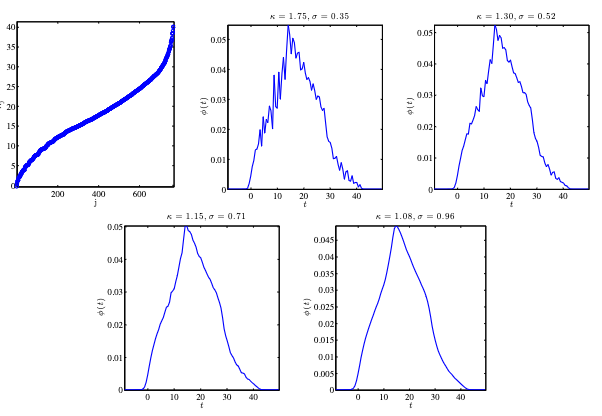
\includegraphics[height=7.5cm]{./Bilder/screenshot.png}

\section{Die Bedingung der Nicht-Negativität}
Als Wahrscheinlichkeitsverteilung ist die Spektraldichte nicht-negativ, also
$$\forall g \in \SR, g \geq 0: \langle \phi, g \rangle \geq 0$$
Einige numerische Annäherungen brechen mit dieser Eigenschaft, darunter auch die Kernel-Polynom-Methode.
Das führt zu großen Fehlern und muss daher unbedingt beachtet werden.
Methoden, um diese negativen Effekte einzudämmen, würden den Rahmen dieser Arbeit aber deutlich überschreiten.